\documentclass[letterpaper, 12pt]{article}

\usepackage{geometry}
 \geometry{
 letterpaper,
 total={170mm,257mm},
 left=20mm,
 top=20mm,
 bottom=20mm
 }
\usepackage{graphicx} % Required for inserting images
\usepackage{authblk}
\usepackage{amssymb}
\usepackage{lipsum}
\usepackage{float}
\usepackage{times}
\usepackage{amsmath}
\usepackage[format=plain,
            labelfont={bf,it},
            textfont=it]{caption}
\captionsetup{justification=raggedright,singlelinecheck=false}
\usepackage{ragged2e}
\usepackage{longtable}
\usepackage{comment}
\usepackage{setspace}
\usepackage{fancyhdr}
\usepackage{titlesec}
\usepackage[hyperindex,breaklinks]{hyperref}
\hypersetup{
    colorlinks=true,
    linkcolor=blue,
    filecolor=magenta,      
    urlcolor=blue,
    pdftitle={Overleaf Example},
    pdfpagemode=FullScreen,
    }
% \usepackage{background} % add COSIG logo to page
\usepackage[T1]{fontenc}
\usepackage{helvet}
\renewcommand{\familydefault}{\sfdefault}
\pagenumbering{gobble}
\usepackage[skip=10pt plus1pt, indent=40pt]{parskip}

\titlespacing*{\section}
{0pt}{1.5ex plus 1ex minus .2ex}{1.3ex plus .2ex}

\renewcommand\Authfont{\fontsize{12}{14.4}\selectfont}
\renewcommand\Affilfont{\fontsize{9}{10.8}\itshape}
 
\begin{document}
\flushleft

\includegraphics[width=0.5\textwidth]{img/home/241017_final_logo_mockup.png}

\section*{Plagiarism of text}
\addcontentsline{toc}{section}{Plagiarism of text}
\textit{Last updated: 29 March 2025}

Plagiarism is the act of copying someone else's work, possibly with minor alterations, and passing it off as one's own work.

High-profile allegations of plagiarism in scholarly works make the news regularly, such as those of a \href{https://www.theguardian.com/education/2024/jan/06/harvard-claudine-gay-plagiarism}{Harvard president} and a \href{https://www.bbc.com/news/world-europe-12504347}{German defense minister}. Cases of plagiarism in Russian academia and politics are frequently uncovered by members of the \href{https://dissernet.org/}{Dissernet} community. Similarly, the \href{https://vroniplag.fandom.com/de/wiki/Home}{VroniPlag wiki} covers German plagiarism cases. These cases often concern works that predate the Internet and modern plagiarism detection tools.

\subsection*{Expected quotation and attribution behavior}

When exactly quoting another publication, authors should put quotation marks around the entirety of the quoted text. The original source should be properly referenced with an in-text citation and an entry in the quoting article's bibliography. Where text is paraphrased from another source, this original source should also be cited. See the \href{https://osf.io/zpf4r}{COSIG entry on citations}.

\subsection*{Simple plagiarism: copied text}

Copying text from another source without quotation marks or without proper attribution is the simplest form of plagiarism. Longer stretches of copied text are generally considered more severe infractions of publication ethics. Text that appears very similar to a prior work for a stretch than a single sentence may arise by mistake (e.g., an author writes a sentence forgetting that they read that exact wording elsewhere) or by coincidence (short statements and phrases may appear in multiple texts simply because there is a limit on the number of ways they may be paraphrased).

\subsection*{Inappropriate text recycling}

Inappropriate text recycling describes the practice of republishing all or part of one's own work with proper attribution or acknowledgment of the previously-published version. Inappropriate text recycling is often referred to as ``self plagiarism'', but text recycling should not be confused for plagiarism. As stated by \href{https://textrecycling.org/files/2021/06/Understanding-Text-Recycling_A-Guide-for-Researchers-V.1.pdf}{Hall et al. (2021) for the Text Recycling Research Project}:


\begin{quote}
    \textit{Policies and guidelines that address text recycling often use the term ``self-plagiarism''. However, that term is confusing. Unlike plagiarism, text recycling doesn’t involve taking someone else's work or ideas and passing them off as your own. Also, unlike plagiarism, there is wide agreement that reuse of your own materials is sometimes acceptable. To avoid these inaccurate implications, the term text recycling is now widely preferred.}
\end{quote}

Inappropriate text recycling often takes the form of the same article being published by the same authors in two different outlets, commonly described as ``dual publication'' or ``duplicate publication''. Most journals will not allow a manuscript to be submitted to multiple journals simultaneously and will not publish work that has previously appeared in another journal.

It is very common (often expected) for scientists to publish work both as a part of their thesis/dissertation as well as in a peer-reviewed journal. This is normally not problematic, although some journals require authors to disclose this and other journals ban the practice outright, considering the thesis a ``prior publication''. 

\subsection*{Plagiarism detection tools and ``plagiarism scores''}

Modern plagiarism detection software, such as those sold by \href{https://www.grammarly.com/plagiarism-checker}{Grammarly}, \href{https://www.turnitin.com/}{Turnitin} and \href{https://www.ithenticate.com/}{iThenticate} compare some input text to a large database of published and online texts to automatically identify portions of text that have been copied. Most large publishers employ one of these automated tools on submitted manuscripts. These tools are useful for detecting simple plagiarism involving copying of text, but may fail for the more complex cases described below. Automated tools typically return a ``plagiarism score'' (more accurately described as a ``text-matching score'' or ``similarity score''), often the percentage of the input text that matches other texts. This score is intended to help humans make a judgment call, not to be used as an objective metric, yet it is frequently misused.

This percentage is rarely zero. These tools will often pick up the titles of cited works, the name of the venue in the headers or footers and other such constructs that are unoriginal by definition and include them in the returned score. Sometimes, the input text will return a high text-matching score for completely benign reasons (e.g., the input text is an article based on a chapter in the author's previously-published thesis). Text-matching scores should never be used in isolation and any suspected plagiarism should always be evaluated by a human assessor.

Some venues explicitly put thresholds on tool-assisted plagiarism detection, such as requiring any submissions to return a plagiarism score below 15\% with Turnitin. An automated plagiarism check is no substitute for a robust editorial and review process. Any publishing outlet that openly advertises that submissions must meet a specific plagiarism score threshold is likely predatory and should be approached with caution.

Knowing that most publishers will use some form of automated plagiarism detection software, paper mills and similar education fraud firms will often offer access to these tools for a fee. This gives their clientele an additional opportunity to conceal their plagiarism if their manuscript does not score well.

\begin{figure}[h!tbp]
    \centering
    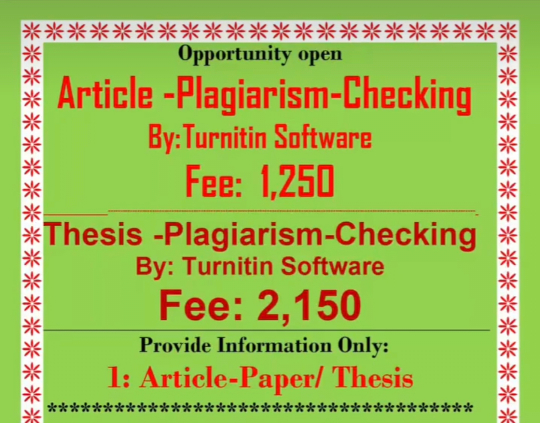
\includegraphics[width=0.5\textwidth]{img/plagiarism/Screenshot_20250328_132930_Instagram.jpg}
    \caption*{A December 10, 2024 advertisement posted on a paper mill's Instagram profile offering to submit customers' articles and theses to Turnitin for a fee.}
\end{figure}

\subsection*{Complex plagiarism: tortured phrases}

Authors who know that their work will be checked for plagiarism often try to hide it by making lots of small changes to the plagiarized text.
For instance, they may replace some words with synonyms, change the punctuation or interweave plagiarized sentences with their own.

Covering up plagiarism is often accomplished with automated paraphrasing software like those offered by \href{https://www.grammarly.com/}{Grammarly} and \href{https://quillbot.com/}{QuillBot}. These tools typically replace words and phrases in the input text with synonyms.
However, because technical works use lots of context-specific jargon, the synonyms found in a thesaurus may not be synonyms in the scientific sense.

Automated plagiarism avoidance thus creates \href{https://doi.org/10.48550/arXiv.2107.06751}{\textbf{tortured phrases}},
phrases that are devoid of scientific meaning and are often not even grammatically correct.
For instance, ``bosom peril'' is a tortured version of ``breast cancer'',
while ``computer getting to know'' is a tortured version of ``machine learning''. More instances of tortured phrases and their expected counterparts are shown in the table below.

\begin{center}
\begin{tabular}{c|c}
    Tortured phrase & Expected phrase \\ \hline\hline
     \href{https://pubpeer.com/search?q=%220.33-celebration%22}{0.33-celebration} & third party  \\ \hline
     \href{https://pubpeer.com/search?q=%22amino%20corrosive%22}{amino corrosive} & amino acid  \\ \hline
     \href{https://pubpeer.com/search?q=%22attractive%20reverberation%22}{attractive reverberation} & magnetic resonance  \\ \hline
     \href{https://pubpeer.com/search?q=%22man-made%20brainpower%22}{man-made brainpower} & artificial intelligence \\ \hline
     \href{https://pubpeer.com/search?q=%22condition%20of-workmanship%22}{condition-of-workmanship} & state-of-the-art \\ \hline
     \href{https://pubpeer.com/search?q=%22inexhaustible%20force%22%20AND%20%22renewable%20energy%22}{inexhaustible force} & renewable energy \\ \hline
     \href{https://pubpeer.com/search?q=%22bogus%20up-sides%22}{bogus up-sides} & false positives \\ \hline
     \href{https://pubpeer.com/search?q=%22message-just%22}{message-just} & text-only \\ \hline
     \href{https://pubpeer.com/search?q=%22underground%20creepy%20crawly%20state%22}{underground creepy-crawly state} & ant colony \\ \hline
     \href{https://pubpeer.com/search?q=%22vitality%20utilization%22}{vitality utilization} & energy use \\ \hline
     \href{https://pubpeer.com/search?q=%22Walk+2020%22}{Walk 2020} & March 2020 \\ \hline
\end{tabular}
\end{center}

One common variant on tortured phrases is the \href{10.1126/science.znqe1aq}{tortured acronynm}.
For instance, if the original paper contains ``Artificial Intelligence (AI)'',
a tortured version might contain ``man-made consciousness (AI)'',
retaining the acronym because the software has no concept of acronyms and thus cannot replace it.
Even proper nouns can be replaced if they are also a common noun, leading to absurdities like \href{https://pubpeer.com/publications/059D502827972226591FC5F5421221}{``Glove Romney''} replacing the name of the American politician Mitt Romney (this particular tortured phrases has also appeared \href{https://web.archive.org/web/20250322132615/https://www.amazon.com/Mitt-Romney-Biography-Book-Flexibility-ebook/dp/B0CLKZKKQG}{outside of scientific articles}).

The \href{https://www.irit.fr/~Guillaume.Cabanac/problematic-paper-screener}{Problematic Paper Screener (PPS) Tortured Phrases Detector} documents thousands of instances of tortured phrases by regularly searching the scientific literature for known tortured phrases.
Newcomers to sleuthing and post-publication peer review should consider looking through the PPS Tortured Phrases Detector for entries that have not yet been assessed by a human and follow the instructions to report the problem on PubPeer.

Tortured phrases are rarely found in isolation; if there is one tortured phrase in an article, there are likely several. When reading a paper with tortured phrases, you may encounter terms the PPS did not detect but that also look like tortured phrases. Look any suspicious phrases up in a scholarly search engine like \href{https://scholar.google.com}{Google Scholar} or \href{https://www.dimensions.ai/}{Dimensions} to see if the phrase has been used in legitimate contexts previously. If not, use the PPS Feedback tool to suggest adding your findings to the tortured phrase database. New tortured phrases can also be identified by taking established scientific terms (e.g., \href{https://doi.org/10.1007/11559573_65}{``Hahn moments''}), substituting in common synonyms and querying the resulting term in these database (\href{https://pubpeer.com/search?q=%22Hahn%20instants%22}{``Hahn instants''})

The presence of tortured phrases in an article implies 1) that parts of the article were plagiarized and 2) that the article was not genuinely peer-reviewed before publication.
No serious editor or peer reviewer would accept a paper purporting to detect ``bosom peril'' using ``man-made consciousness''.
Venues that publish such works likely publish numerous other problematic articles.

\subsection*{Complex plagiarism: translation}

Authors may plagiarize another work by translating text out of its original language and into another. This often results in non-standard grammatical structures and nonsensical sentences.

\subsection*{Detecting plagiarism and finding originals}

Simple plagiarism can often be detected by gut instinct alone. For instance, while reading a text, you may notice that

\begin{itemize}
    \setlength\itemsep{-0.5em}
    \item The tone of the text suddenly changes.
    \item Identical concepts are suddenly referred to with wildly different vocabulary.
    \item A poorly-written manuscript suddenly switches to perfect grammar and spelling.
\end{itemize}

The best proof that text has been plagiarized is identification of the original source from which the text was plagiarized. This is much easier to accomplish for instances of simple plagiarism than for paraphrased or translated plagiarized text. For simple plagiarism, looking up one of the anomalous sentences in a search engine often brings up its source.

Finding the original text from a tortured text boils down to guessing which parts of a text have been replaced, guessing what the original words were and searching for the possible original words (see Example 2 below).

\begin{comment}
Looking for words that \emph{aren't} tortured can be useful if they are unique enough that they help narrow down the search.
\end{comment}

It is important to provide evidence that the ``original'' source predates the ``plagiarized'' version.
This can be indicate with publication or submissions dates, or other details such as the original having high-resolution versions of figures that are blurry in the copy.

\subsection*{Example 1: Simple plagiarism}

\href{https://doi.org/10.1155/2007/48242}{Cimini et al. (2007)} report on the expression of different proteins during neural stem cell differentiation. The first two paragraphs in the Introduction section of this article are nearly identical to the prior article by \href{https://doi.org/10.1016/j.plipres.2005.12.002}{Feige et al. (2006)}. This article was \href{https://doi.org/10.1155/2019/5656198}{retracted in 2019} with a retraction notice describing plagiarism and image manipulation. 

\subsection*{Example 2: Tortured phrases, original source identified}

\href{https://doi.org/10.1016/j.gltp.2021.01.002}{Alshari and Gawali (2021)} describe a technique for land-use land cover (LULC) classification. The text of the article is filled with tortured phrases. One section titled ``Hybrid approach'' begins with ``A mixture approach joins the upsides of the computerized and manual strategies to create a land cover map that is in a way that is better than if a solitary technique was available''. The section title is a hint that the original text used the word ``hybrid'' instead of ``mixture''. One might also guess that ``upsides'' should read ``advantages'' and ``computerized'' should read ``automated''. Sure enough, querying a search engine for \verb|"hybrid approach" + "advantages of the automated and manual"| returns the original text, from \href{https://www.amnh.org/content/download/74344/1391366/file/land-cover-classification-methods.pdf}{Horning (2004)}: ``A hybrid approach combines the advantages of the automated and manual methods to
produce a land cover map that is better than if just a single method was used''.

\subsection*{Example 3: Translation plagiarism, original source identified}

\href{https://doi.org/10.1111/mbe.12345}{Sadvakassova et al. (2022)} describe techniques to manage the stress of preschool students with special needs. The text, in English, is frequently nonsensical, apparently plagiarized from another work by \href{https://cyberleninka.ru/article/n/harakteristika-trevozhno-fobicheskogo-sostoyaniya-u-detey-doshkolnogo-vozrasta-s-zaderzhkoy-psihicheskogo-razvitiya-kak}{Klimova (2010)}, written in Russian. The article was retracted in 2023.

\begin{figure}[h!tbp]
    \centering
    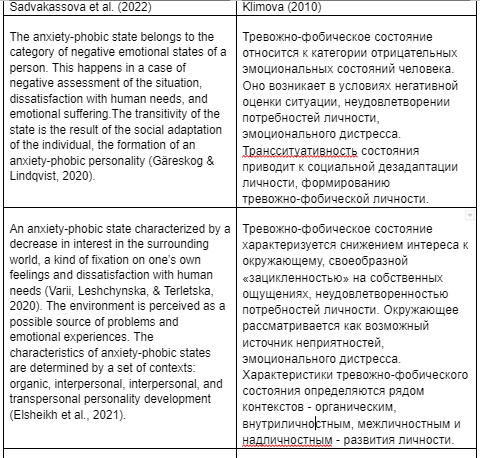
\includegraphics[width=0.8\textwidth]{img/plagiarism/image-1697289264849.png}
    \caption*{A comparison of the English text by \href{https://doi.org/10.1111/mbe.12345}{Sadvakassova et al. (2022)} to the Russian text by \href{https://cyberleninka.ru/article/n/harakteristika-trevozhno-fobicheskogo-sostoyaniya-u-detey-doshkolnogo-vozrasta-s-zaderzhkoy-psihicheskogo-razvitiya-kak}{Klimova (2010)}. Citations are added to the translated text that were not present in the original. Figure created by \href{https://pubpeer.com/publications/A6C5007F7D6DF81B20F72098A04F20\#2}{Anna Abalkina}.}
\end{figure}

\subsection*{Example 4: Duplicate publication, translated}

\href{https://doi.org/10.1007/978-3-319-51859-6_14}{Garz\'on et al. (2017)} describe a new material for greenhouses in an English-language book chapter. This chapter was \href{https://doi.org/10.1007/978-3-319-51859-6_20}{retracted in 2021} because the work was \href{https://ingenieriacivil.cedex.es/index.php/ingenieria-civil/article/view/521}{previously published} by some of the same authors in Spanish.

\pagebreak

\subsection*{Additional resources}

\begin{itemize}
    \setlength\itemsep{-0.5em}
    \item \href{https://www.ox.ac.uk/students/academic/guidance/skills/plagiarism}{Guide on plagiarism for Oxford University students}
    \item \href{https://doi.org/10.24318/cope.2019.2.2}{COPE: Plagiarism in a published article}
    \item \href{https://doi.org/10.48550/arXiv.2107.06751}{``Tortured phrases: A dubious writing style emerging in science. Evidence of critical issues affecting established journals'' (2021)}
    \item \href{https://doi.org/10.1007/978-3-030-46711-1_2}{``Disguised academic plagiarism: Translation plagiarism'' (2018)}
    \item \href{https://doi.org/10.1007/s10503-019-09481-3}{``The Pernicious Effects of Compression Plagiarism on Scholarly Argumentation'' (2019)}
    \item \href{https://ori.hhs.gov/self-plagiarism}{Self plagiarism guide from United States Department of Health and Human Service Office of Research Integrity}
    \item \href{https://textrecycling.org/}{Text Recycling Research Project}
\end{itemize}

\end{document}